\section{Bài 2: HTTP}
Xóa cache browser trước khi truy cập trang web hoặc dùng ẩn danh. Dùng Wireshark để bắt gói tin khi truy cập vào website: http://example.com.\\
Việc bắt gói tin bằng Wireshark trong bài được thực hiện bằng \textbf{máy ảo}, sử dụng hệ điều hành \textbf{Windows Server 2012 R2}.\\
Kết quả bắt gói tin chi tiết được lưu trong tập tin \textbf{\textit{bai2.pcapng}}.

\textbf{1. Chụp hình kết quả bắt gói tin từ lúc bắt đầu DNS đến lúc gửi HTTP request (thấy được những gói tin liên quan).}
\begin{figure}[H]
\begin{center}
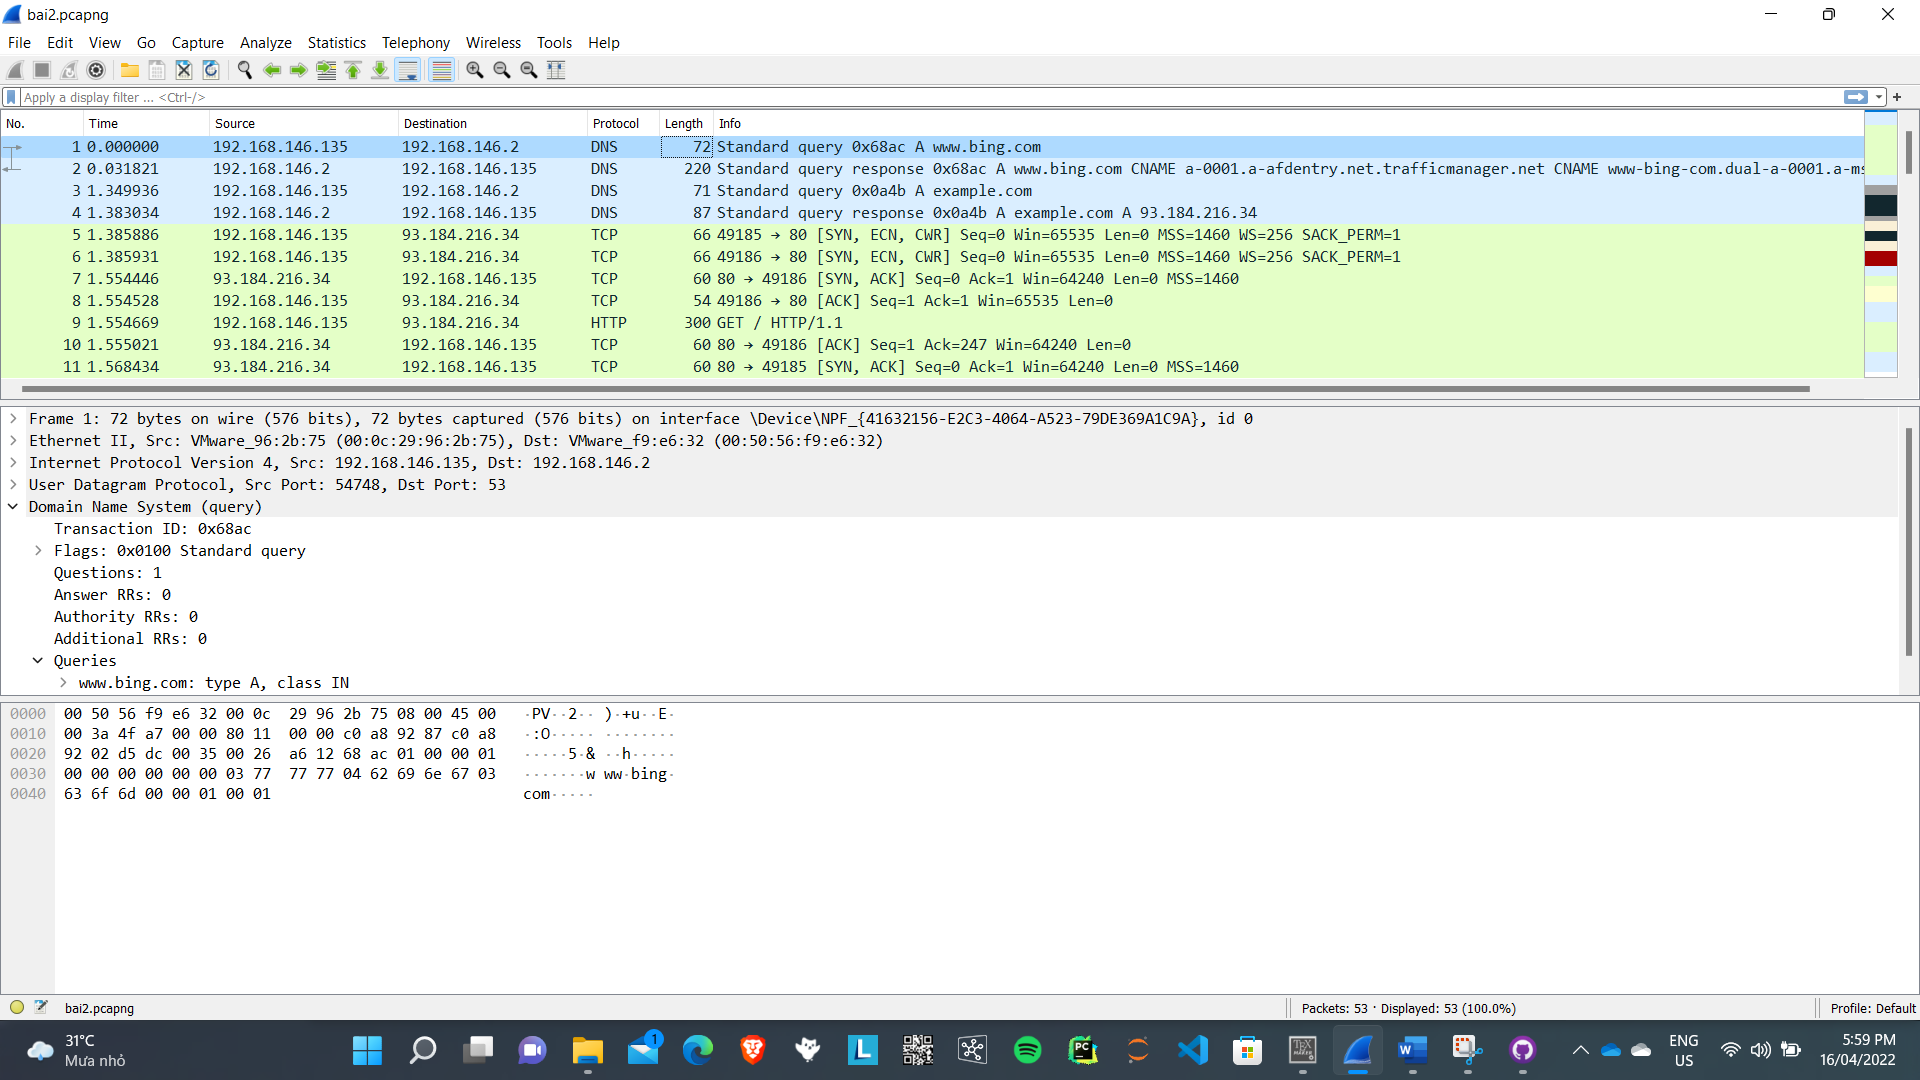
\includegraphics[scale=.45]{../figures/p2/p2_intro}
\end{center}
\caption{Kết quả bắt gói tin từ lúc bắt đầu DNS đến lúc gửi HTTP request}
\end{figure}

\textbf{2.	Cho biết IP của host.}\\
IP của host là: 192.168.146.35.
\begin{figure}[H]
\begin{center}
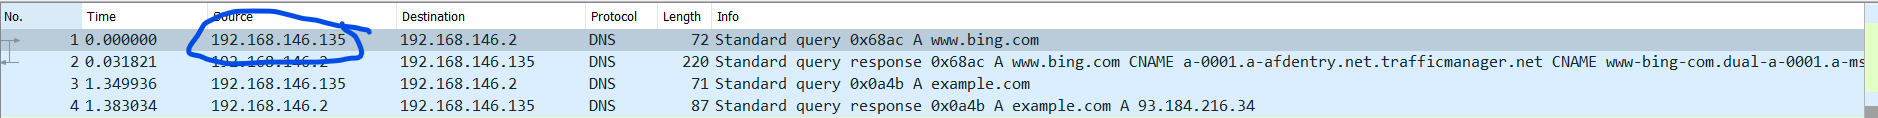
\includegraphics[scale=1]{../figures/p2/p2_hostip}
\end{center}
\caption{Địa chỉ IP của host}
\end{figure}

\textbf{3. Cho biết IP của router (default gateway) (nếu không thấy được thì trả lời không có và giải thích tại sao)}\\
IP của router là: \textbf{192.168.146.2}.
\begin{figure}[H]
\begin{center}
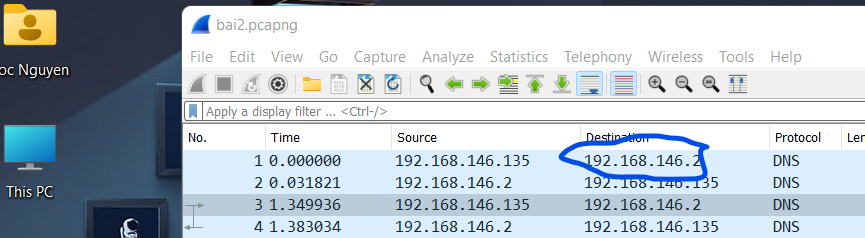
\includegraphics[scale=1]{../figures/p2/p2_routerip}
\end{center}
\caption{Địa chỉ IP của router}
\end{figure}

\textbf{4. Cho biết địa chỉ MAC của host.}\\
Địa chỉ MAC của host là: \textbf{00:0c:29:96:2b:75}.
\begin{figure}[H]
\begin{center}
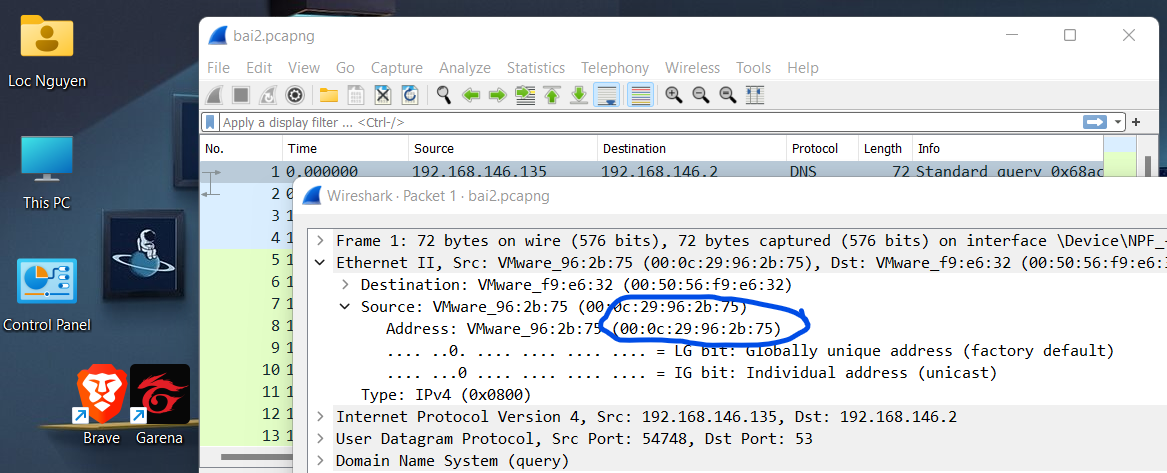
\includegraphics[scale=1]{../figures/p2/p2_hostmac}
\end{center}
\caption{Địa chỉ MAC của host}
\end{figure}

\textbf{5.	Cho biết địa chỉ MAC của router (default gateway).}\\
Địa chỉ MAC của router là: \textbf{00:50:56:f9:e6:32}.
\begin{figure}[H]
\begin{center}
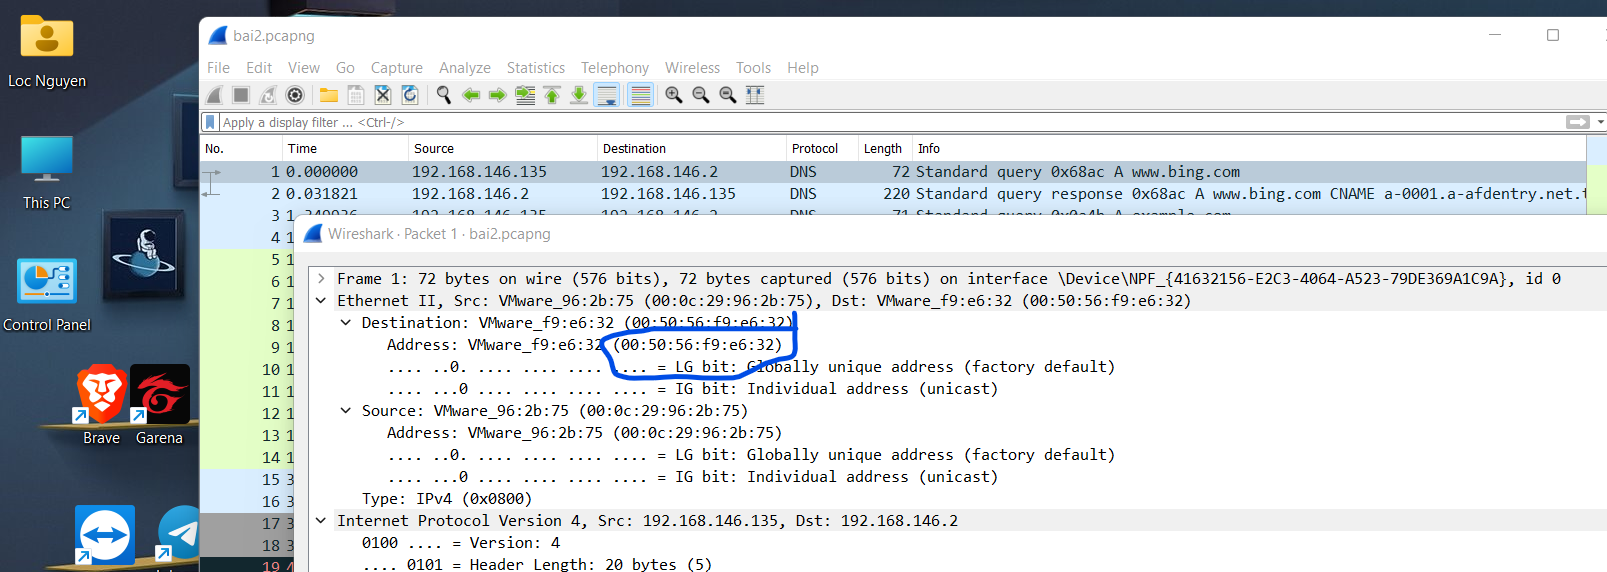
\includegraphics[scale=1]{../figures/p2/p2_routermac}
\end{center}
\caption{Địa chỉ MAC của router}
\end{figure}

\textbf{6.	Protocol nào được sử dụng để phân giải tên miền của trang web?}\\
Protocol được dùng để phân giải tên miền của trang web: \textbf{DNS}.
\begin{figure}[H]
\begin{center}
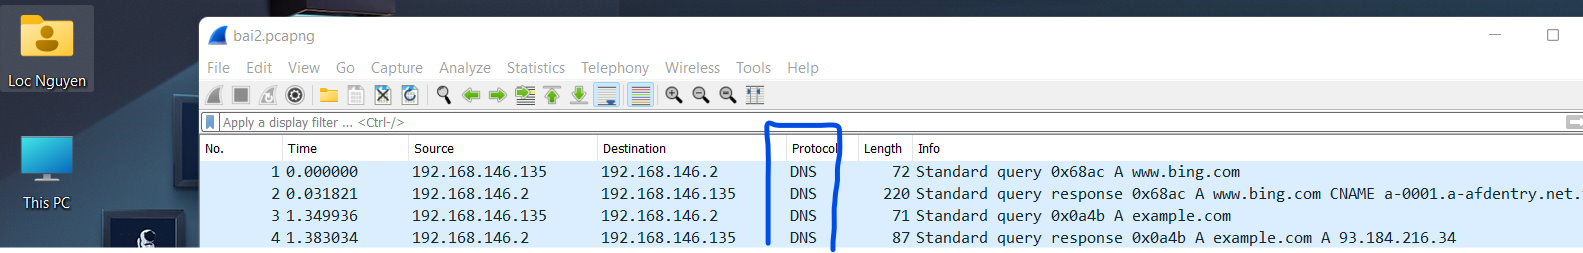
\includegraphics[scale=1]{../figures/p2/p2_protocol1}
\end{center}
\caption{Protocol phân giải tên miền}
\end{figure}

\textbf{7.	Cho biết IP của HTTP server.}\\
Địa chỉ IP của HTTP server là: \textbf{93.184.216.34}.
\begin{figure}[H]
\begin{center}
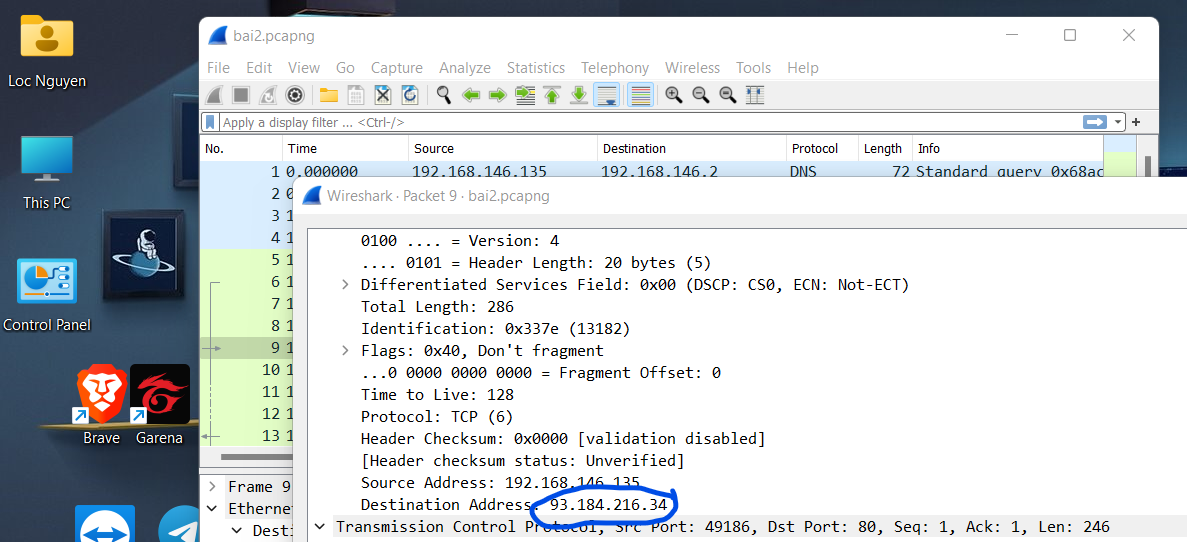
\includegraphics[scale=1]{../figures/p2/p2_httpserverip}
\end{center}
\caption{Địa chỉ IP của HTTP server}
\end{figure}

\textbf{8.	Cho biết protocol của tầng Transport được sử dụng bởi DNS.}\\
DNS sử dụng protocol \textbf{UDP} của tầng Transport.
\begin{figure}[H]
\begin{center}
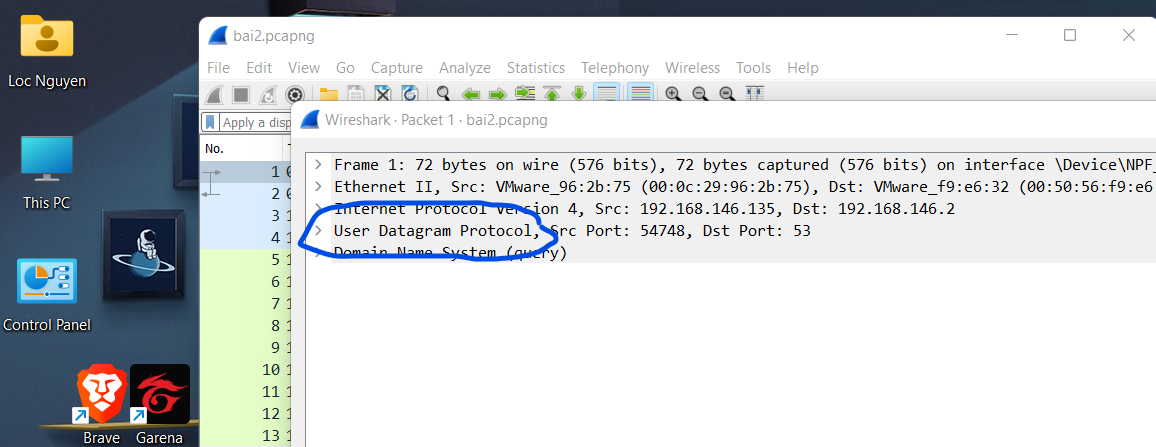
\includegraphics[scale=1]{../figures/p2/p2_dnsprotocol}
\end{center}
\caption{Nghi thức được DNS sử dụng}
\end{figure}

\textbf{9.	Cho biết port sử dụng khi truy vấn DNS server.}\\
Port sử dụng khi truy vấn DNS server: \textbf{port 53.}
\begin{figure}[H]
\begin{center}
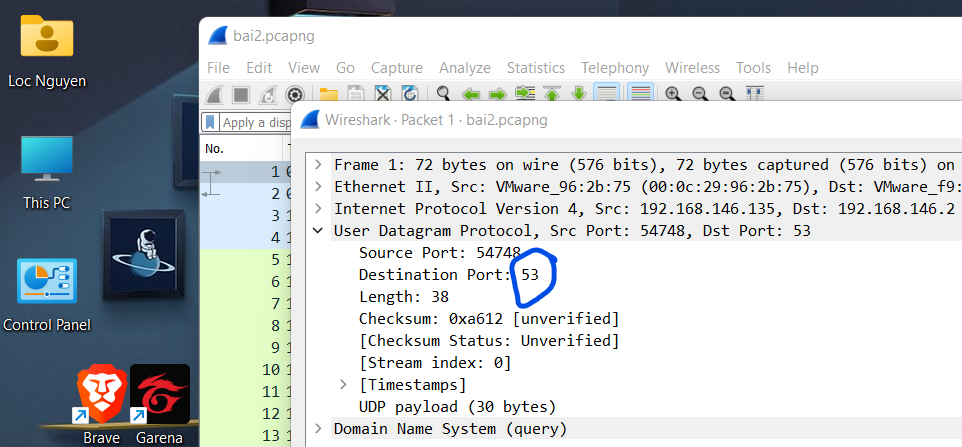
\includegraphics[scale=1]{../figures/p2/p2_dnsport}
\end{center}
\caption{Port sử dụng khi truy vấn DNS server}
\end{figure}

\textbf{10. Bao lâu thì quá trình bắt tay 3 bước (3-way handshake) hoàn thành?}
Thời gian quá trình 3-way handshake hoàn thành: \textbf{0.168597000 giây.}
\begin{figure}[H]
\begin{center}
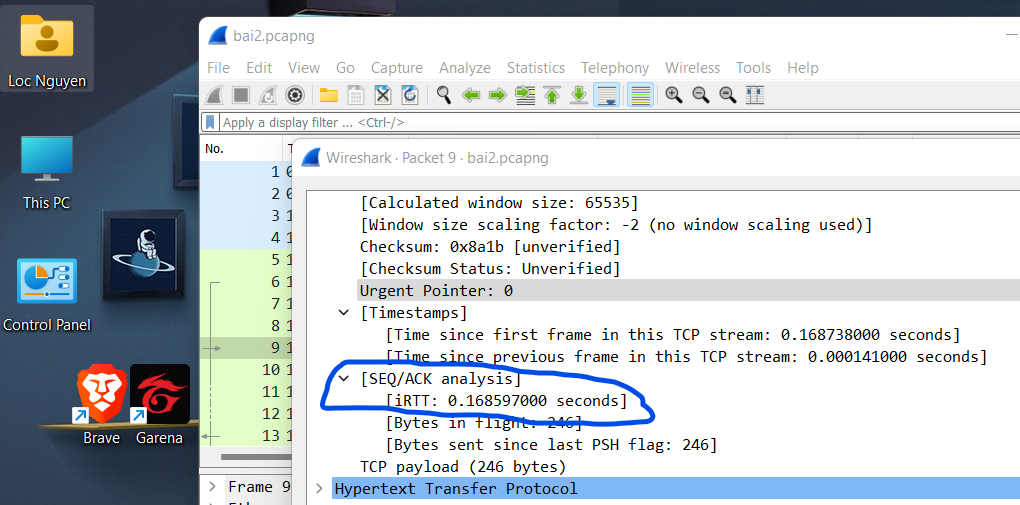
\includegraphics[scale=1]{../figures/p2/p2_handshake}
\end{center}
\caption{Thời gian hoàn thành quá trình 3-way handshake}
\end{figure}

\textbf{11.	 Cho biết host machine của website đang truy cập (Application - host field)}\\
Host machine của website đang truy cập là: \textbf{example.com}.

\textbf{12. Cho biết version HTTP mà trình duyệt web (bowser) đang sử dụng (Application).}\\
Version HTTP mà trình duyện web đáng sử dụng là: \textbf{HTTP/1.1}.
\begin{figure}[H]
\begin{center}
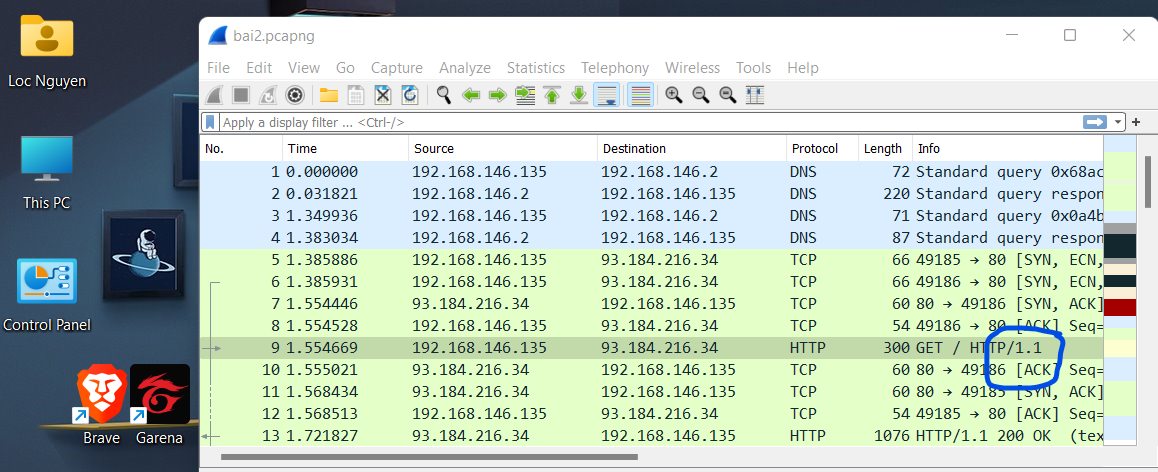
\includegraphics[scale=1]{../figures/p2/p2_httpversion}
\end{center}
\caption{Version HTTP}
\end{figure}

